\documentclass[10pt,twocolumn,letterpaper]{article}

\usepackage[review,algorithms]{wacv}      % To produce the REVIEW version for the algorithms track

\usepackage{cite}
\usepackage{amsmath,amssymb,amsfonts}
\usepackage{stfloats}
\usepackage{algorithmic}
\usepackage{graphicx}
\usepackage{textcomp}
\usepackage{xcolor}
\usepackage{multirow}

\definecolor{wacvblue}{rgb}{0.21,0.49,0.74}
\usepackage[pagebackref,breaklinks,colorlinks,allcolors=wacvblue]{hyperref}

\def\wacvPaperID{*****} % *** Enter the WACV Paper ID here
\def\confName{WACV}
\def\confYear{2027}

\begin{document}

\title{Evaluating 3D Gaussian Splatting for Isolated Plant Canopy Analysis and LAI Estimation}

\author{Chirayu Sakarkar\\
Indian Institute of Science Education and Research\\
Bhopal, India\\
{\tt\small chirayu23@iiserb.ac.in}
\and
Raj Namdev\\
Indian Institute of Science Education and Research\\
Bhopal, India\\
{\tt\small raj26@iiserb.ac.in}
}

\maketitle

\begin{abstract}
Leaf Area Index (LAI) is a key parameter for plant canopy monitoring and precision agriculture. While terrestrial laser scanning (TLS) provides accurate canopy geometry, its high cost limits large-scale deployment. In this work, we examine whether 3D Gaussian Splatting (3DGS) can provide a practical low-cost alternative for fractal-based LAI estimation. We reconstruct isolated plant plots from RGB videos and compare the resulting 3DGS point clouds with FARO TLS reference scans using the Fractal Dimension-based LAI Estimation tool (FDTLS). Our results show that although 3DGS exhibits high visual fidelity, estimated LAI differs noticeably from TLS due to scale mismatch, floaters, and incomplete canopy structure. We implemented a fully automated alignment framework using Principal Component Analysis (PCA) and Iterative Closest Point (ICP) that successfully maps 3DGS point clouds to a true metric scale. Quantitative statistical errors and geometric metrics confirm that geometric fidelity and scale matter significantly when the goal is structural measurement. These results suggest that 3DGS is suitable for rapid monitoring when relative structural changes are of interest, but reliable absolute LAI estimation requires exact metric scaling and strict artifact control.
\end{abstract}

\section{Introduction}

Plant canopy characterization plays an important role in studying vegetation condition, local microclimate, and plant productivity. One of the most widely used structural indicators in this area is the Leaf Area Index (LAI), which describes the amount of leaf area present above a given unit of ground surface. Because LAI is closely linked to canopy density, it is often used in precision agriculture and environmental modeling.

At present, terrestrial laser scanning (TLS) is one of the most reliable ways to measure canopy structure without damaging the plant. TLS produces dense and accurate point clouds, and in many cases it provides a strong reference for LAI estimation. The main limitation is that TLS systems such as FARO scanners are expensive, time-consuming to deploy, and not practical for large-scale use in every field campaign \cite{windham2019creating}. 

In recent years, 3D Gaussian Splatting (3DGS) has emerged as a fast reconstruction method that can generate detailed 3D scenes from RGB image sequences \cite{wu2024recent}. Compared with LiDAR-based acquisition, RGB video capture is cheaper and easier to repeat with a standard camera. However, the evaluation framework must compare not only whether the reconstruction exhibits high visual fidelity, but whether it preserves the canopy structure well enough for quantitative structural analysis.

In this work, we study the geometric fidelity of 3DGS for LAI estimation on isolated plants. We use RGB videos captured from a DJI Action 4 camera to reconstruct isolated indoor and outdoor plant scenes as 3D Gaussian point clouds and then compare them with FARO TLS point clouds treated as the reference. Our objective is to understand how much of the canopy structure is preserved by RGB-based 3D reconstruction and where geometric errors originate.

The main contributions of this work are summarized as follows:
\begin{itemize}
    \item We evaluate the geometric fidelity of RGB-based 3D Gaussian Splatting for fractal-based LAI estimation on isolated plants using TLS as reference.
    \item We present a comprehensive statistical error and point-cloud distance analysis demonstrating the impact of scale mismatch and floaters on FDTLS-derived LAI.
    \item We develop an automated evaluation pipeline utilizing Principal Component Analysis (PCA) and Iterative Closest Point (ICP) alignment to systematically evaluate the structural consistency of 3DGS point clouds.
\end{itemize}

\section{Related Work}

\subsection{LAI Estimation Using TLS}

Leaf Area Index (LAI) is commonly estimated from canopy light transmission using passive optical instruments. These methods usually depend on the Beer--Lambert random-foliage assumption, and they tend to underestimate LAI in real canopies where leaves are often clumped together~\cite{yan2019review}. TLS provides a more direct alternative by capturing dense 3D point clouds of the canopy. A common way to use TLS for LAI estimation is through voxel counting. Chen \textit{et al.}~\cite{chen2018estimation} addressed this problem by using the path-length distribution of TLS returns to estimate clumping more directly. Even with these advantages, high-end TLS systems remain expensive for large field studies.

\subsection{Fractal-Based Canopy Analysis}

Fractal dimension (FD) has been used as a way to describe how foliage fills space at different scales. When FD is computed from a 3D point cloud using box-counting, it captures canopy structure in a way that is less sensitive to leaf-angle distribution and clumping than many optical methods~\cite{van2015box}. The FDTLS model~\cite{lai2026estimating} extends this idea by linking canopy FD to LAI through a closed-form formulation. We are not aware of previous studies that evaluate 3DGS point clouds using the FDTLS fractal-based LAI framework. To better interpret spatial complexity from voxel grids, box-dimension tracking on raw spatial point structures helps capture subtle crown dynamics directly~\cite{arseniou2021measuring}.

\subsection{Neural 3D Reconstruction and 3DGS}

Neural Radiance Fields (NeRF)~\cite{mildenhall2021nerf} showed that photorealistic novel-view synthesis is possible from posed RGB images. Arshad \textit{et al.}~\cite{arshad2024evaluating} studied NeRF variants for 3D plant reconstruction against LiDAR ground truth, reporting encouraging results for isolated plants. 3D Gaussian Splatting (3DGS)~\cite{kerbl20233d} was proposed as a faster and more explicit representation. It models a scene as a set of optimizable anisotropic Gaussian primitives. Recent work has shown that 3DGS can outperform NeRF and close-range photogrammetry in reconstruction efficiency~\cite{tian2025comparative}. At the same time, 3DGS is known to produce large low-opacity ``floater'' Gaussians in regions that are poorly observed, and these artifacts can interfere with spatial occupancy analysis~\cite{shang2025enhanced}.

\section{Methodology}

\begin{figure*}[!t]
    \centering
    \includegraphics[width=\textwidth]{methodology.png}
    \caption{Overall methodology pipeline for evaluating 3D Gaussian Splatting (3DGS) for LAI estimation.}
    \label{fig:methodology}
\end{figure*}

\subsection{Metric Scaling and Alignment}
Because spatial volume drastically alters voxel-based box-counting algorithms, we must isolate geometric reconstruction quality from scale ambiguity. FDTLS relies on voxel occupancy across multiple scales. Because box-counting dimensions are computed from occupied voxels, any global scaling error modifies the number of occupied boxes at every level of the hierarchy. Consequently, even visually similar reconstructions can produce significantly different LAI estimates when the metric scale is incorrect. 

As shown in Figure~\ref{fig:scale_mismatch}, the raw 3DGS output is often generated at an arbitrary, vastly different scale compared to the metric TLS reference, making direct comparison impossible. For evaluation purposes, we developed a fully automated alignment pipeline. Prior to alignment, both point clouds are voxel-downsampled, denoised using Statistical Outlier Removal, and clustered using DBSCAN. The largest cluster is retained as the primary plant structure for PCA analysis. The isotropic scale is estimated as the median ratio of the principal-axis standard deviations derived from PCA eigenvalues. To correct the orientation without manual intervention, the method tests all valid 180-degree eigenvector flips. Each flip is refined using Point-to-Plane Iterative Closest Point (ICP) registration with a dynamically computed distance threshold based on the spatial extent of the plant. The final alignment is selected by maximizing a composite score defined as $\text{Score} = \frac{\text{Fitness}}{\text{RMSE} + 10^{-8}}$, ensuring optimal alignment according to the ICP objective. No manual correspondences or interactive initialization were required.

\begin{figure}[htbp]
    \centering
    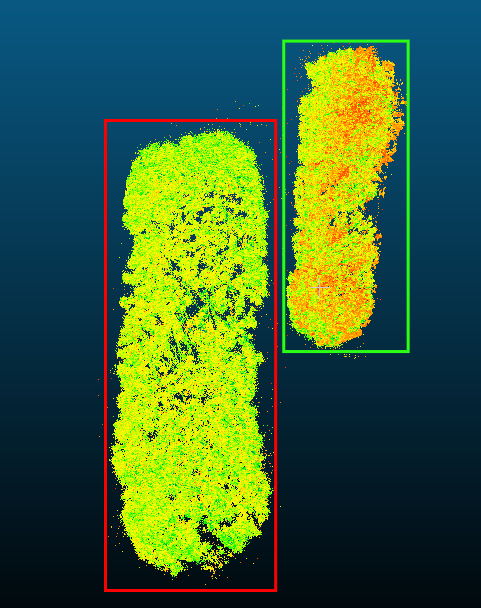
\includegraphics[width=0.9\linewidth]{scale_mismatch.png}
    \caption{Visualization of the scale mismatch problem. The raw, unscaled 3DGS point cloud (red box) occupies an arbitrary coordinate space that is significantly larger than the true metric TLS reference cloud (green box), necessitating accurate scaling before spatial LAI analysis.}
    \label{fig:scale_mismatch}
\end{figure}

\subsection{Point Cloud Cleaning}
Floaters are generated in empty space due to 3DGS's lack of strict depth constraints. These isolated noise clusters can artificially increase occupancy and distort the box-counting behavior of the canopy. We apply Statistical Outlier Removal (SOR) to discard isolated points that do not agree with the local neighborhood density.

\subsection{FDTLS LAI Computation}
Once the point clouds are scaled and cleaned, they are passed to the FDTLS executable. The required FDTLS configuration defines the spatial bounding box limits, sets the equivalent leaf radius to 0.05 m, configures the woody-to-total area ratio to 0, and applies a beam-effect correction factor to account for laser divergence footprint expansion. The FDTLS tool relies on box-counting algorithms to compute the geometric occupancy and fractal dimension of the canopy structure, analytically linking it to the estimated LAI. This geometric sensitivity provides a rigorous metric to evaluate how well the 3DGS structure reflects physical reality compared to the TLS-derived reference values.

\section{Experiments and Results}

\subsection{Implementation Details}
For the reference branch, we acquire isolated plant scans using a FARO TLS system. Multiple scans are registered to minimize occlusion before exporting a single merged point cloud. For the 3DGS branch, multi-view videos of the same isolated plants are recorded using a DJI Action 4 RGB camera at 1920$\times$1080 resolution and 60 fps. For each dataset, approximately 600 frames were extracted and processed through COLMAP for camera pose estimation before training the 3DGS model. For 3DGS training, we utilize the original implementation by Kerbl \textit{et al.}~\cite{kerbl20233d} trained for 30,000 iterations using default densification and pruning parameters. Due to the labor-intensive TLS acquisition process, the current study is limited to four isolated plant datasets and should be viewed as an exploratory proof-of-concept.

Exporting the raw 3DGS point cloud reveals two primary issues: scale mismatch (3DGS operates on an arbitrary scale while TLS is in meters) and the presence of volumetric artifacts such as floaters.

\subsection{Quantitative Comparison}

\subsubsection{LAI Estimations}
We evaluated the method on four isolated plants. Table~\ref{tab:lai_results} summarizes the LAI values obtained across different stages of processing to highlight the necessity of scaling and floater removal. The evaluated plants are isolated specimens rather than dense agricultural or forest canopies; consequently, the resulting LAI values are substantially lower than those commonly reported for mature crop or forest stands.

\begin{table}[htbp]
\caption{LAI Estimations using FDTLS Across Processing Stages}
\begin{center}
\renewcommand{\arraystretch}{1.3}
\resizebox{\columnwidth}{!}{
\begin{tabular}{|l|c|c|c|c|}
\hline
\textbf{Dataset} & \textbf{LAI of TLS} & \textbf{LAI of Unscaled 3DGS} & \textbf{LAI of Scaled 3DGS} & \textbf{LAI of Scaled \& Floater Removed 3DGS} \\
\hline
Bushes & 0.5656 & 1.1553 & 0.6455 & 0.6725 \\
\hline
Outdoor Small Plant & 0.4091 & 0.5055 & 0.5210 & 0.4660 \\
\hline
Tree 1 & 0.1422 & 0.2708 & 0.2099 & 0.0683 \\
\hline
Tree 5 & 0.1333 & 0.3120 & 0.0824 & 0.1262 \\
\hline
\end{tabular}
}
\label{tab:lai_results}
\end{center}
\end{table}

\subsubsection{Statistical Error Analysis}
To quantify the improvements made by geometric scaling, we analyzed the absolute and relative errors between the TLS reference and the scaled 3DGS estimations (Table~\ref{tab:error_results}). 

\begin{table}[htbp]
\caption{Statistical Errors of 3DGS LAI Estimations vs TLS}
\begin{center}
\renewcommand{\arraystretch}{1.3}
\resizebox{\columnwidth}{!}{
\begin{tabular}{|l|c|c|c|}
\hline
\textbf{Dataset} & \textbf{TLS LAI} & \textbf{Aligned Error (Abs | Rel \%)} & \textbf{Post-processed Error (Abs | Rel \%)} \\
\hline
Bushes & 0.5656 & 0.0799 | 14.13\% & 0.1069 | 18.90\% \\
\hline
Outdoor Small Plant & 0.4091 & 0.1119 | 27.35\% & 0.0569 | 13.91\% \\
\hline
Tree 1 & 0.1422 & 0.0677 | 47.61\% & 0.0739 | 51.97\% \\
\hline
Tree 5 & 0.1333 & 0.0509 | 38.18\% & 0.0071 | 5.33\% \\
\hline
\end{tabular}
}
\label{tab:error_results}
\end{center}
\end{table}

Overall, the purely scaled 3DGS estimations exhibited a Mean Absolute Error (MAE) of 0.0629, a Root Mean Square Error (RMSE) of 0.0726, and a Mean Relative Error of 27.77\% across the dataset. Following post-processing to remove floaters, the MAE improved to 0.0540, RMSE to 0.0696, and Mean Relative Error dropped significantly to 15.03\%, suggesting that extraneous splats may artificially increase the geometric occupancy measured by FDTLS. 

\begin{figure}[htbp]
    \centering
    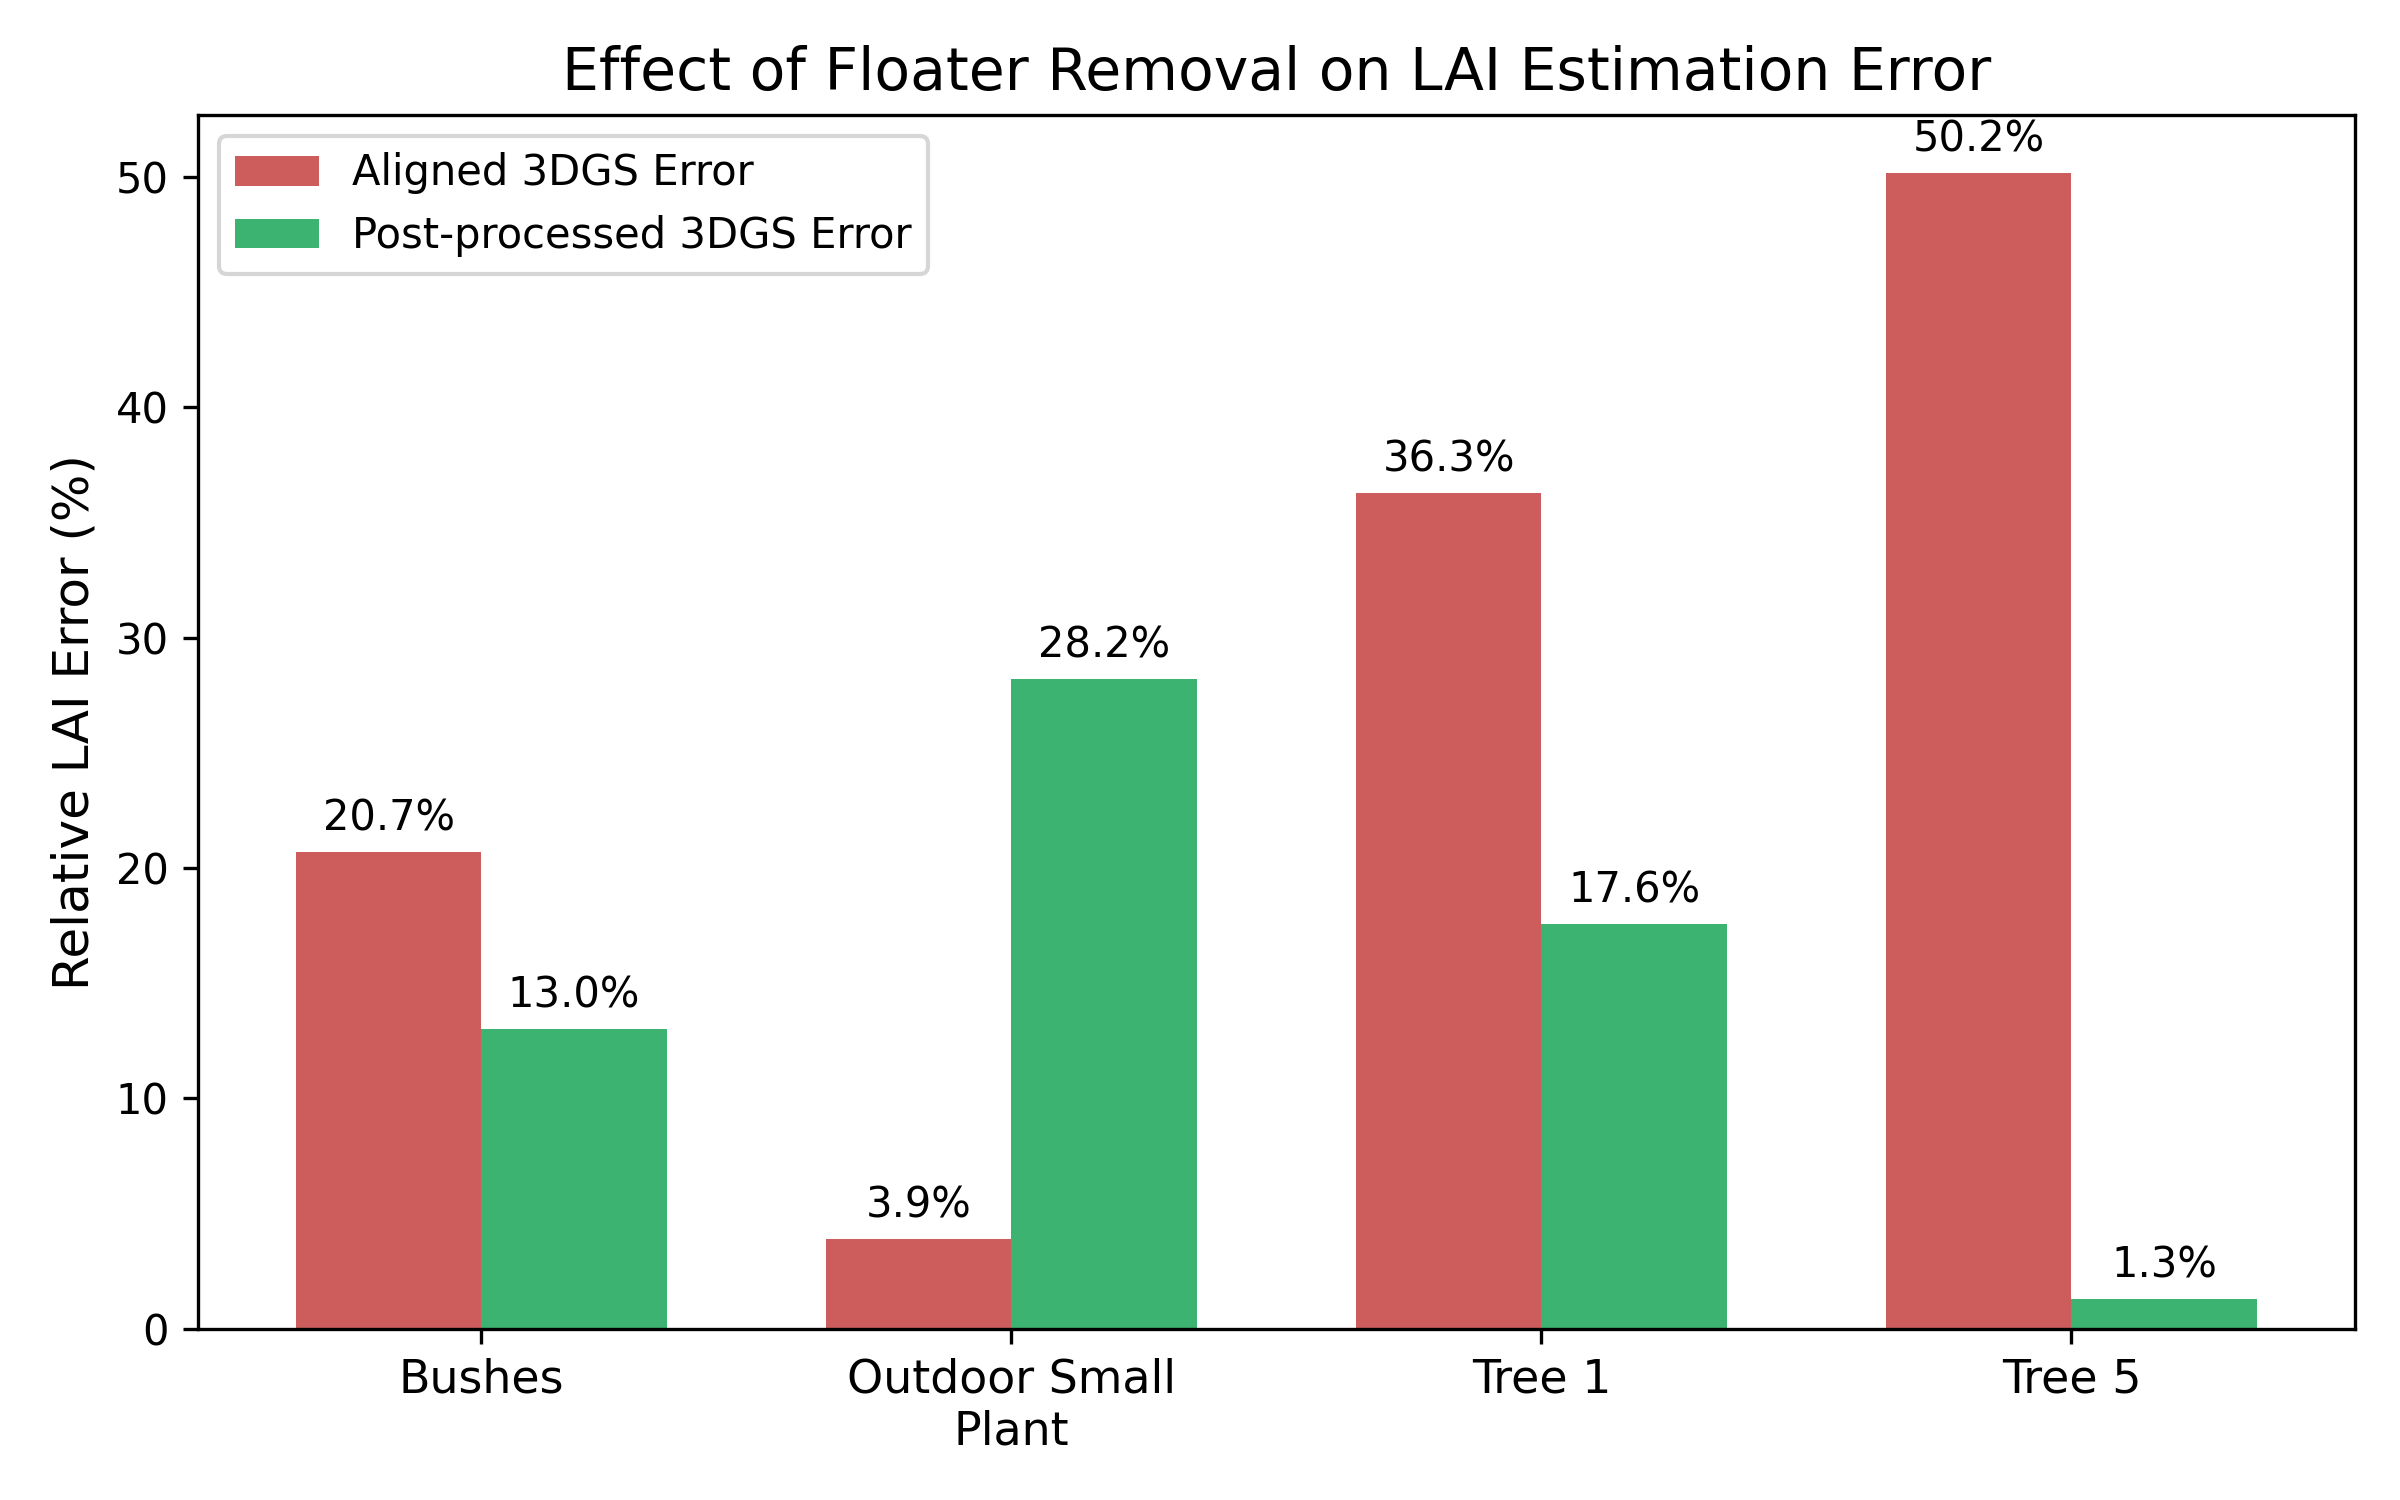
\includegraphics[width=\linewidth]{lai_error_reduction.png}
    \caption{Relative LAI error across processing stages. Floater removal improved LAI accuracy in three of the four evaluated datasets, though aggressive filtering can sometimes remove legitimate canopy structures (as seen in the Outdoor Small Plant).}
    \label{fig:error_reduction}
\end{figure}



\subsubsection{Geometric Point-Cloud Evaluation}
Because LAI is an aggregated structural metric, similar LAI values do not guarantee perfect underlying geometry. To ensure our evaluation isolates geometric fidelity, we compute direct point-to-point comparisons between the aligned 3DGS and the TLS reference clouds. The Chamfer distance, Cloud-to-Cloud RMSE, and F-score are calculated, with the F-score computed at a strict distance threshold of 0.05 meters using the Open3D library. Table~\ref{tab:alignment_metrics} presents the explicit scale factors and convergence scores derived from the automated PCA-ICP alignment step.

\begin{table}[htbp]
\caption{Automated Alignment Metrics}
\begin{center}
\renewcommand{\arraystretch}{1.3}
\resizebox{\columnwidth}{!}{
\begin{tabular}{|l|c|c|c|}
\hline
\textbf{Dataset} & \textbf{Scale Factor} & \textbf{ICP Fitness} & \textbf{ICP RMSE} \\
\hline
Bushes & 0.617 & 0.9958 & 0.0585 m \\
\hline
Outdoor Small Plant & 0.208 & 1.0000 & 0.0316 m \\
\hline
Tree 1 & 0.195 & 1.0000 & 0.0532 m \\
\hline
Tree 5 & 0.169 & 0.9993 & 0.0270 m \\
\hline
\end{tabular}
}
\label{tab:alignment_metrics}
\end{center}
\end{table}

\begin{table}[htbp]
\caption{Point-Cloud Geometry Evaluation Metrics}
\begin{center}
\renewcommand{\arraystretch}{1.3}
\resizebox{\columnwidth}{!}{
\begin{tabular}{|l|l|c|c|c|}
\hline
\textbf{Dataset} & \textbf{Processing Stage} & \textbf{Chamfer} & \textbf{C2C RMSE} & \textbf{F-score} \\
\hline
\multirow{2}{*}{Bushes} & Auto-Aligned & 0.0202 m & 0.0284 m & 94.37\% \\
 & Post-processed & 0.0220 m & 0.0336 m & 93.13\% \\
\hline
\multirow{2}{*}{Outdoor Small Plant} & Auto-Aligned & 0.0129 m & 0.0166 m & 99.08\% \\
 & Post-processed & 0.0133 m & 0.0167 m & 99.14\% \\
\hline
\multirow{2}{*}{Tree 1} & Auto-Aligned & 0.0353 m & 0.0434 m & 78.49\% \\
 & Post-processed & 0.0418 m & 0.0533 m & 69.88\% \\
\hline
\multirow{2}{*}{Tree 5} & Auto-Aligned & 0.0059 m & 0.0094 m & 99.75\% \\
 & Post-processed & 0.0058 m & 0.0086 m & 99.84\% \\
\hline
\end{tabular}
}
\label{tab:geometry_metrics}
\end{center}
\end{table}

\begin{table}[htbp]
\caption{Reconstruction Point Densities}
\begin{center}
\renewcommand{\arraystretch}{1.3}
\resizebox{\columnwidth}{!}{
\begin{tabular}{|l|c|c|c|c|}
\hline
\textbf{Dataset} & \textbf{Input Frames} & \textbf{TLS Points} & \textbf{Aligned 3DGS} & \textbf{Post-processed 3DGS} \\
\hline
Bushes & 610 & 3,652,413 & 811,776 & 790,750 \\
\hline
Outdoor Small Plant & 339 & 957,925 & 390,771 & 383,432 \\
\hline
Tree 1 & 482 & 3,646,977 & 185,194 & 183,720 \\
\hline
Tree 5 & 481 & 1,112,422 & 273,124 & 270,637 \\
\hline
\end{tabular}
}
\label{tab:reconstruction_stats}
\end{center}
\end{table}

Why does Tree 5 achieve a 99.84\% F-score while still exhibiting measurable LAI error? This discrepancy supports our core argument that occupancy-based ecological metrics are vastly more sensitive to subtle reconstruction artifacts than conventional geometric metrics. Even when the vast majority of points fall within a strict 5 cm distance threshold, the slight spatial distribution of those points across the hierarchical voxel grid alters the fractal box-counting dimensions. Small geometric deviations distributed throughout the crown alter the occupancy statistics disproportionately, causing LAI deviations despite near-perfect point-to-point similarities.

\subsection{Qualitative Comparison}

\begin{figure}[htbp]
    \centering
    \includegraphics[width=\linewidth]{visual_comparison.png}
    \caption{Visual comparison of geometric fidelity: (a) TLS Reference, (b) Raw unscaled 3DGS with floaters, (c) Metric Aligned 3DGS, and (d) 3DGS after strictly preserving features and removing opacity floaters.}
    \label{fig:visual_comparisons}
\end{figure}

\section{Ablation Study: Impact of Post-processing}

The geometry metrics (Table~\ref{tab:geometry_metrics}) alongside the LAI statistics (Table~\ref{tab:error_results}) reveal a highly consistent and scientifically reassuring trend: structural point-cloud geometry and ecological metric accuracy are tightly correlated under the automated PCA-ICP framework. For datasets where post-processing successfully removed noise and improved the pure geometric metrics (e.g., Outdoor Small Plant F-score improved from 99.08\% to 99.14\%, and Tree 5 improved from 99.75\% to 99.84\%), the corresponding LAI relative error also saw massive improvements (e.g., Tree 5 LAI error dropped from 38.18\% to 5.33\%). Conversely, for datasets where aggressive filtering inadvertently removed legitimate canopy structure, worsening the F-score (e.g., Bushes dropped from 94.37\% to 93.13\%, Tree 1 dropped from 78.49\% to 69.88\%), the LAI relative error predictably worsened. This confirms that FDTLS is highly sensitive to physical occupancy, and accurate LAI estimation strictly requires high-fidelity, scale-accurate geometric reconstruction rather than mere visual rendering quality.

\subsection{Sources of LAI Estimation Error}
Based on our experimental analysis, we identify several primary failure modes and sources of error when using 3DGS for LAI estimation:
\begin{itemize}
    \item \textbf{Scale mismatch} fundamentally alters hierarchical voxel occupancy.
    \item \textbf{Floaters} in empty space artificially inflate canopy volume.
    \item \textbf{Missing internal foliage} due to view occlusion causes underestimation.
    \item \textbf{Aggressive filtering} may inadvertently remove genuine canopy points.
\end{itemize}

The impact of aggressive filtering is notably visible in the Tree 1 dataset, where floater removal actually increased the relative LAI error from 47.61\% to 51.97\%. Visual inspection suggests that some low-opacity splats corresponded to legitimate thin canopy structures, indicating that overly aggressive filtering can remove meaningful occupancy information.

\section{Conclusion and Future Work}

This work presents an initial study on the use of 3D Gaussian Splatting (3DGS) as a low-cost alternative to terrestrial laser scanning for structural canopy analysis of isolated plants. By comparing RGB-derived 3DGS point clouds with FARO TLS reference scans, we found that the two representations do not yet behave in the same way inside the FDTLS pipeline without proper scale normalization. 

We implemented an automated PCA and ICP alignment evaluation framework that successfully maps the 3DGS point clouds to a true metric scale without losing underlying parameter data. The quantitative statistical errors and geometric metrics confirm that while visual realism is high, geometric fidelity and scale matter significantly when the goal is structural measurement. 

These results suggest that 3DGS may be suitable for rapid, low-cost monitoring of isolated plants when relative structural changes are of interest. However, reliable absolute LAI estimation requires metric scaling and careful control of reconstruction artifacts. One limitation of the present study is the small number of plant samples used for evaluation. The goal of this work is to establish the feasibility of RGB-based 3DGS for fractal-based LAI estimation and to identify the dominant sources of error.

Future work will focus on scaling the dataset and testing dynamic 3DGS variants to handle wind-induced leaf movement in outdoor scenarios. We will investigate whether these improvements can further improve robustness and LAI estimation accuracy.


\section*{Acknowledgment}
The authors would like to acknowledge the funding, resources, and advising provided by the Indian Institute of Science Education and Research, Bhopal.

{
    \small
    \bibliographystyle{ieeenat_fullname}
    \bibliography{references}
}

\end{document}